\documentclass[12pt, a4paper]{article}
\renewcommand*\contentsname{Inhaltsverzeichnis}
\usepackage[ngerman]{babel}
\usepackage{mathptmx}
\usepackage{blindtext}
\usepackage{emptypage}
\usepackage{wrapfig}
\usepackage[pdftex]{graphicx}
\usepackage{geometry}
\usepackage{setspace}
\usepackage{hyperref}
\usepackage[version=4,arrows=pgf-filled,
textfontname=sffamily,
mathfontname=mathsf]{mhchem}
\usepackage[table]{xcolor}
\usepackage{multirow}
\usepackage[table]{xcolor}
\usepackage{array}
\usepackage{float}
\usepackage{mathcomp}
\usepackage{csquotes}
\usepackage{graphicx}
\usepackage{subcaption}
\usepackage[backend=biber,style=chem-acs,sorting=none]{biblatex}
\addbibresource{literatur.bib}  % Deine .bib-Datei einbinden

\DeclareCiteCommand{\cite}
  {\usebibmacro{prenote}}
  {\textsuperscript{\printfield{labelnumber}}}
  {\multicitedelim}
  {\usebibmacro{postnote}}


 \geometry{
 a4paper,
 total={170mm,257mm},
 left=25mm,
 top=25mm,
 }
\setstretch{1.213}


\newcommand{\datum}{\day.\month.\year}
\DeclareGraphicsExtensions{.pdf,.jpeg,.png,.jpg} 

\begin{document}


\begin{figure}
    \includegraphics[scale=0.14]{Universität_Bayreuth.svg.png}
\end{figure}


%Deckblatt

{\raggedright Universität Bayreuth\\  95447 Bayreuth}


\vspace{5cm}

\begin{center}
{\LARGE\bf{Praktikum Anorganische Chemie III}} \\  
\vspace{1cm}
{\Large\bf{Glassherstellung}}\\
\vspace{0.5cm}
{\large Justus Friedrich\\}
{Studiengang: B.Sc. Chemie\\}
{4. Fachsemester}
\end{center}





\thispagestyle{empty}
\begin{center}
{\small Matrikelnummer: 1956010 \\
E–Mail:  bt725206@myubt.de}
\end{center}

\vspace{5cm}

\today


\newpage
%Inhaltsverzeichnis
\tableofcontents
\thispagestyle{empty}


%Teil 1
\newpage
\setcounter{page}{1}
\section{Einleitung}



\subsection{Motivation}
Gläser besitzen in der Regel interessante physikalische und chemische Eigenschaften. Diese resultieren aus ihrer amorph strukturierten Anordnung, 
bei der keine langfristige, regelmäßige Kristallstruktur vorliegt. In diesem Experiment sollen Gläser mit unterschiedlichen Konzentrationen von Netzwerkbildnern und Netzwerkwandlern 
hergestellt werden. Anschließend wird der Verknüpfungsgrad der Netzwerkbildner analysiert, um Rückschlüsse auf die Struktur und Eigenschaften des Glases ziehen zu können. \cite{Skript}

\newpage
%Teil2
\section{Durchführung}
\subsection{Synthese der Verschieden Gläser}
Es werden sieben verschiedene Glaszusammensetzungen hergestellt. Die dafür benötigten Massen der Ausgangsstoffe, um 2 g Glass zu bekommen, werden der Tabelle \ref{Verhältnisse} entnommen. Die jeweiligen Komponenten werden sorgfältig miteinander vermörsert und anschließend in Quarztiegel überführt.
\noindent
Die Proben werden zunächst über 2 Stunden auf 200 °C erhitzt und bei dieser Temperatur für weitere 2 Stunden gehalten. Danach erfolgt eine weitere Aufheizung auf 800 °C über 2 Stunden, gefolgt von einem Halten bei dieser Temperatur für weitere 2 Stunden.
\noindent
Anschließend werden die Gläser durch Abschrecken bei Raumtemperatur (Quenching) verfestigt. Dazu werden sie in einen Exsikkator unter Schutzglas überführt.


\begin{table}[!h]
  \caption{Zeigt die Mol Verhältnisse der Produkte im Glas, und die dafür nötigen Eduktmassen und deren Mol Anzahl. Die Berrechungen für die Mol-Anzahl sind in Gleichung (1) und (2) dargestellt.}
  \begin{center}
    \begin{tabular}{|>{\centering\arraybackslash}p{2.3cm}|>{\centering\arraybackslash}p{1cm}|>{\centering\arraybackslash}p{1cm}|>{\centering\arraybackslash}p{1cm}|>{\centering\arraybackslash}p{1cm}|>{\centering\arraybackslash}p{1cm}|>{\centering\arraybackslash}p{1cm}|>{\centering\arraybackslash}p{1cm}|>{\centering\arraybackslash}p{1cm}|}
      \hline
      \rowcolor{gray}
      \cellcolor{lightgray}Mol\% \ce{Na2O} & 30\% & 35\% & 40\% & 45\% & 50\% & 55\% & 60\% & 70\% \\
      \hline
      \rowcolor{yellow}
       \cellcolor{lightgray}Masse \ce{Na2CO3} [g]&0.54&0.66&0.77&0.90&1.04&1.19&1.35&1.73 \\
      \hline
       \cellcolor{lightgray}Mol \ce{Na2CO3} [mmol]&5.09&6.23&7.26&8.49&9.81&11.2&12.7&16.3 \\
      \hline
      \rowcolor{gray}
       \cellcolor{lightgray}Mol\% \ce{P2O5} & 70\% & 65\% & 60\% & 55\% & 50\% & 45\% & 40\% & 30\% \\
      \hline
      \rowcolor{yellow}      
       \cellcolor{lightgray}Masse \ce{NH4H2PO4} [g]&2.73&2.61&2.51&2.39&2.26&2.11&1.95&2.61 \\
      \hline
       \cellcolor{lightgray}Mol \ce{NH4H2PO4} [mmol]&23.7&22.7&21.8&20.8&19.6&18.34&16.9&13.9 \\
      \hline
    \end{tabular}
  \end{center}

  \label{Verhältnisse}
\end{table}

\subsection{Gleichungen zur Berechnung}
\begin{equation}
  \frac{2 g}{M(\ce{Na2O})+\frac{mol\%  (\ce{P2O5})}{mol\%  (\ce{Na2O})}\cdot M(\ce{P2O5})}= n(\ce{Na2CO3})
\end{equation}

\begin{equation}
  n(\ce{NH4H2PO4})= 2 \cdot n(\ce{Na2CO3})
\end{equation}



\newpage
\section{Auswertung}
\subsection{XRD-Analyse von Glas}
Zunächst werden die XRDs der verschiedenen Gläser betrachtet. Dabei liegt der Fokus auf dem Vergleich der Konzentrationen und den dazugehörigen XRD-Reflexen.

\begin{figure}[h]
\centering

% Erste Zeile (4 Bilder)
\begin{subfigure}[b]{0.23\textwidth}
  \centering
  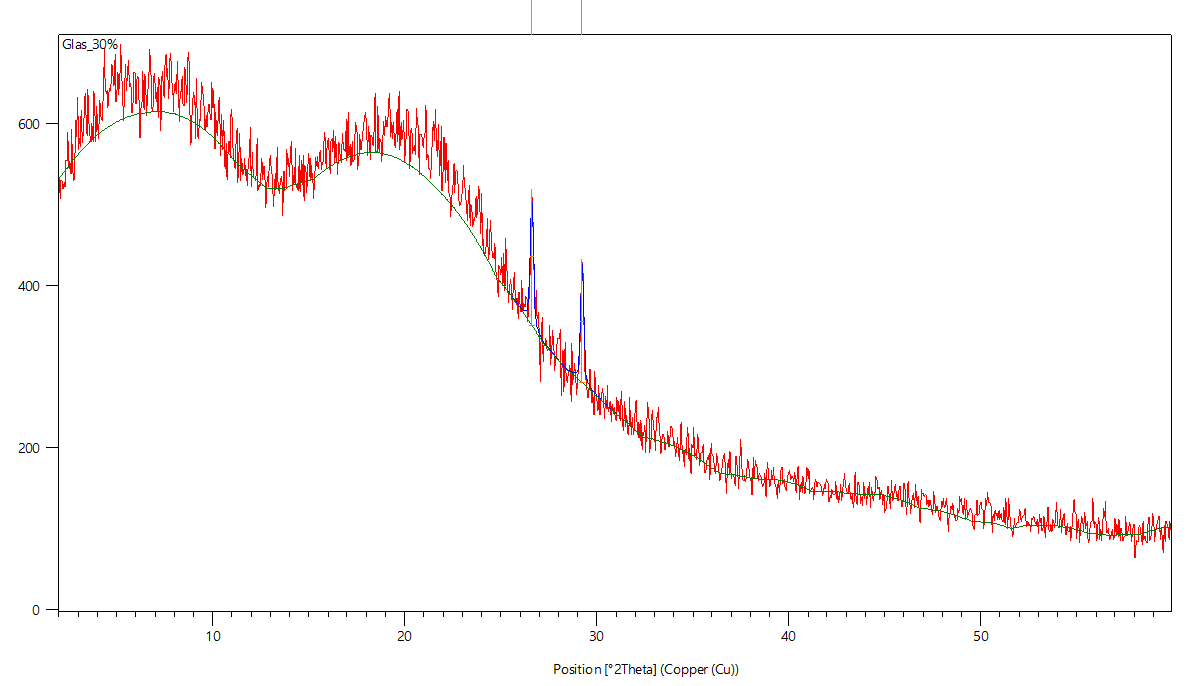
\includegraphics[width=\linewidth]{30pro.png}
  \caption{30 mol \% \ce{Na2O}}
  \label{fig:sub1}
\end{subfigure}
\hfill
\begin{subfigure}[b]{0.23\textwidth}
  \centering
  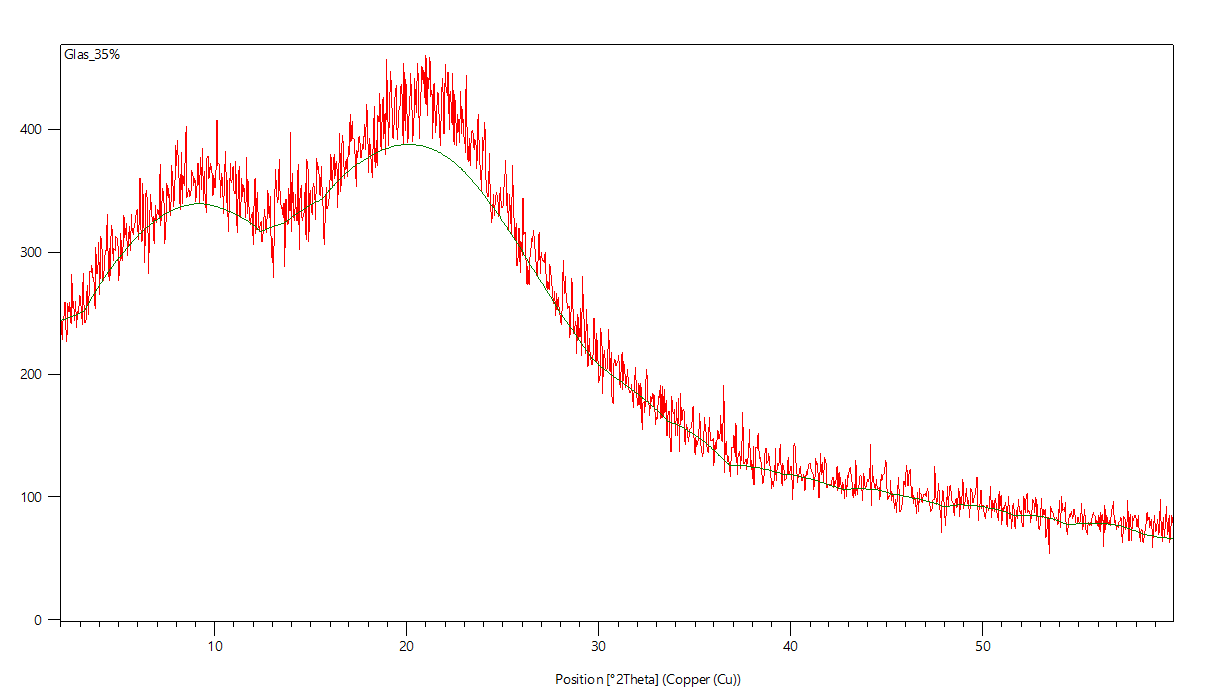
\includegraphics[width=\linewidth]{35pro.png}
  \caption{35 mol \% \ce{Na2O}}
  \label{fig:sub2}
\end{subfigure}
\hfill
\begin{subfigure}[b]{0.23\textwidth}
  \centering
  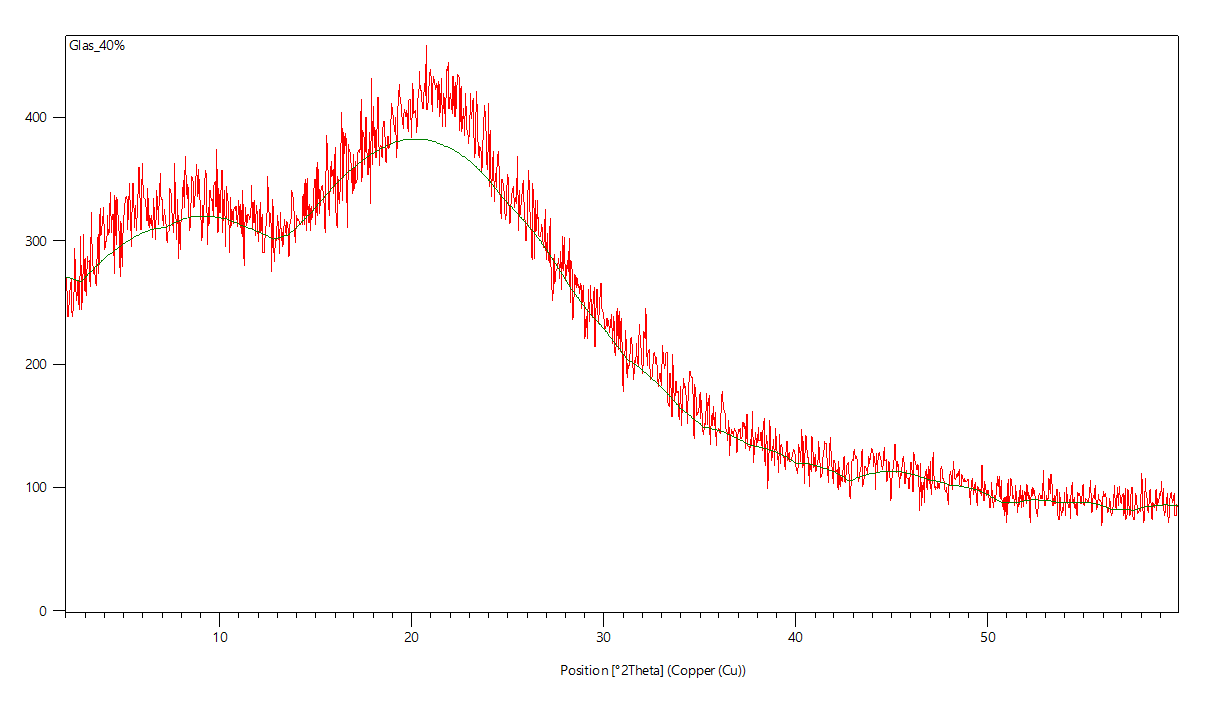
\includegraphics[width=\linewidth]{40pro.png}
  \caption{40 mol \% \ce{Na2O}}
  \label{fig:sub3}
\end{subfigure}
\hfill
\begin{subfigure}[b]{0.23\textwidth}
  \centering
  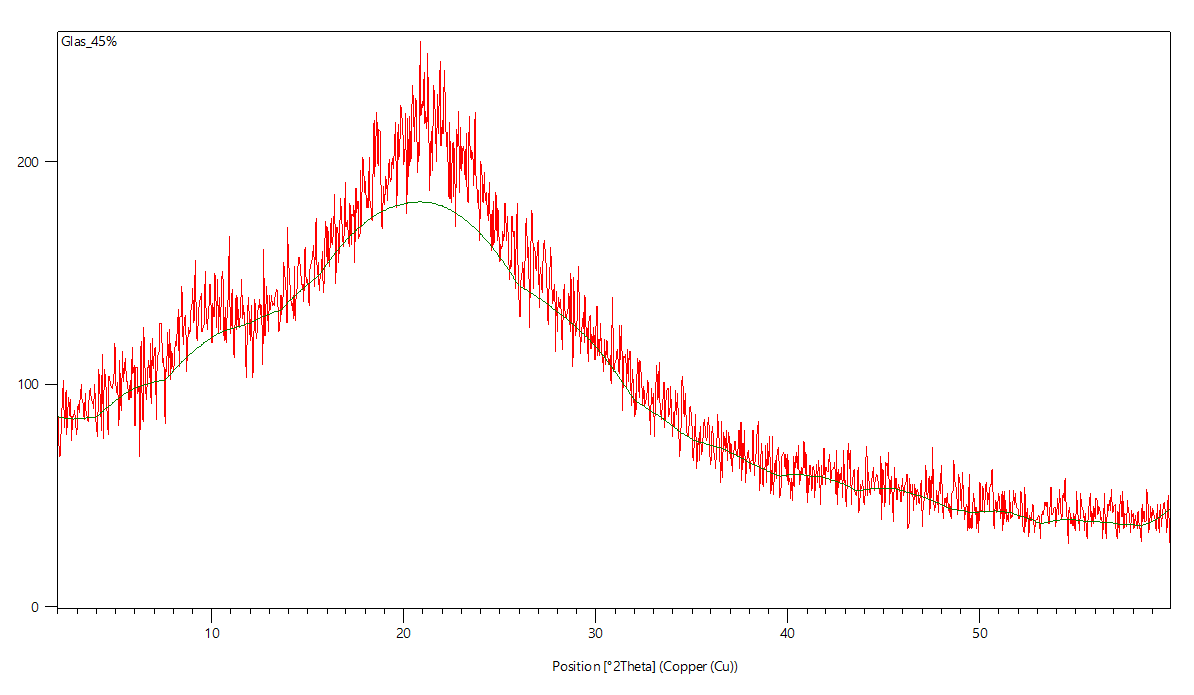
\includegraphics[width=\linewidth]{45pro.png}
  \caption{45 mol \% \ce{Na2O}}
  \label{fig:sub4}
\end{subfigure}

\vspace{0.8em}

% Zweite Zeile (3 Bilder)
\begin{subfigure}[b]{0.3\textwidth}
  \centering
  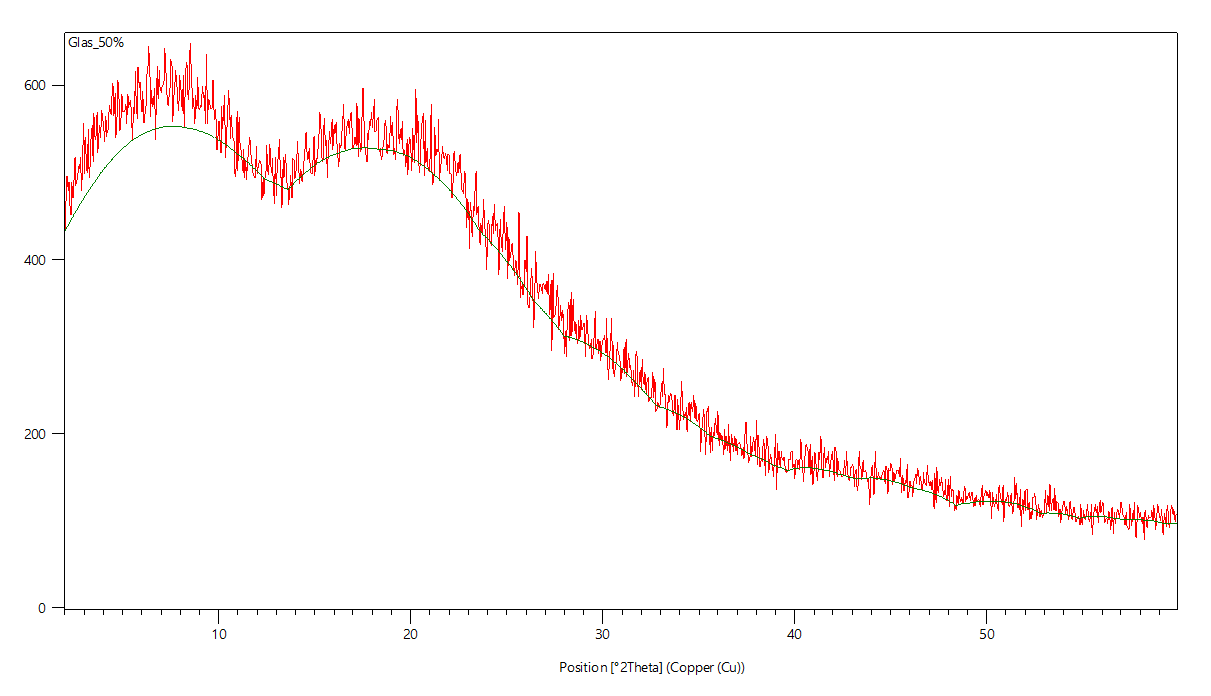
\includegraphics[width=\linewidth]{50pro.png}
  \caption{50 mol \% \ce{Na2O}}
  \label{fig:sub5}
\end{subfigure}
\hfill
\begin{subfigure}[b]{0.3\textwidth}
  \centering
  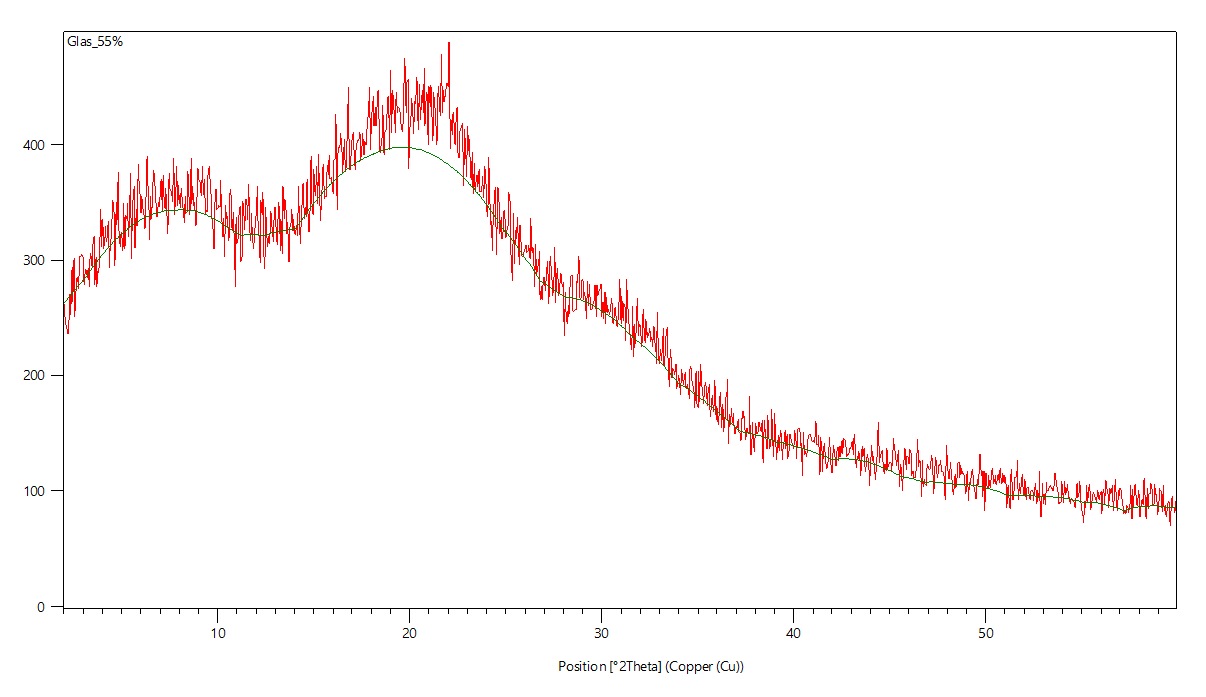
\includegraphics[width=\linewidth]{55pro.png}
  \caption{55 mol \% \ce{Na2O}}
  \label{fig:sub6}
\end{subfigure}
\hfill
\begin{subfigure}[b]{0.3\textwidth}
  \centering
  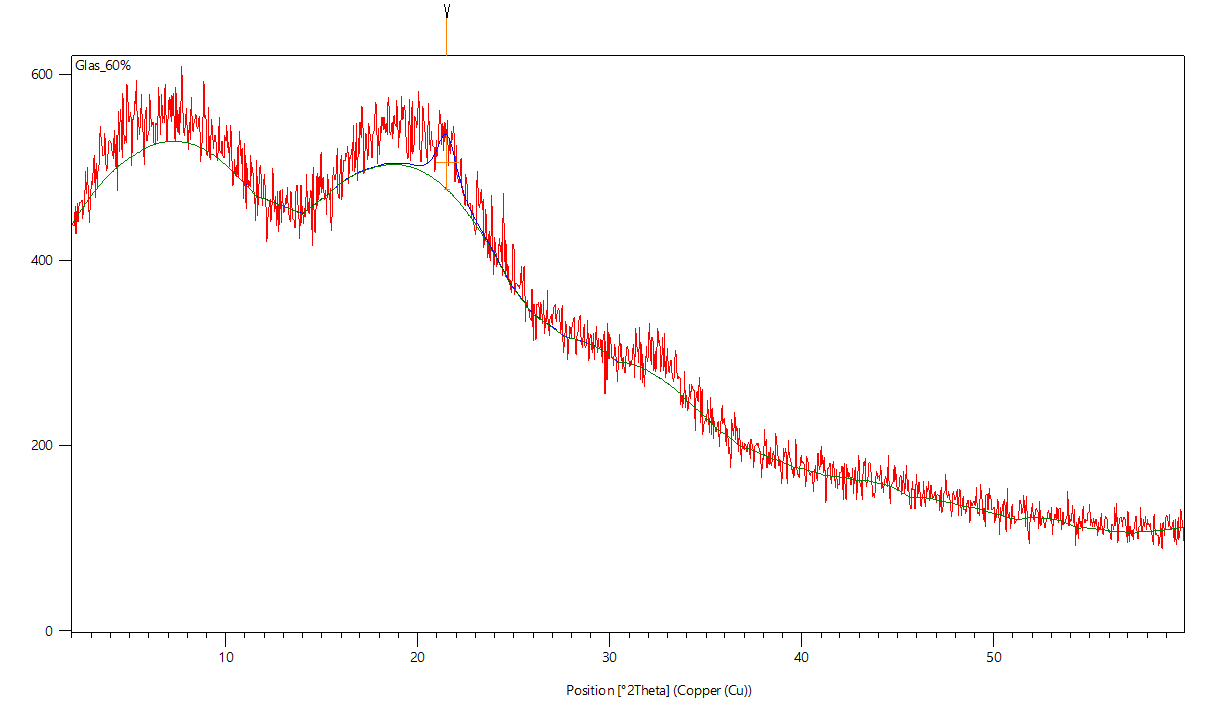
\includegraphics[width=\linewidth]{60pro.png}
  \caption{60 mol \% \ce{Na2O}}
  \label{fig:sub7}
\end{subfigure}

\caption{Zeigt die XRDs von den Verschieden mol \% \ce{Na2O} }
\label{fig:sieben_bilder}
\end{figure}


\begin{figure}[!h]
  \centering
  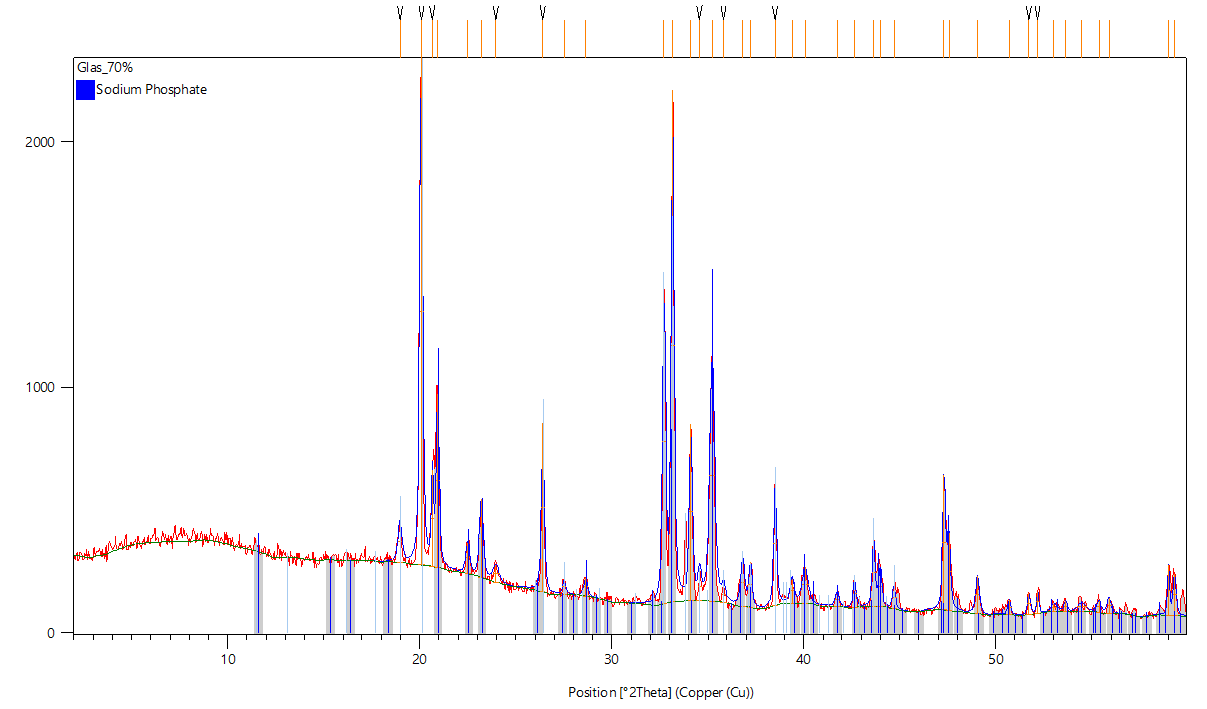
\includegraphics[width=0.90\linewidth]{70pro.png}
  \caption{Zeigt das XRD von dem Glas mit 70 \% \ce{Na2O}, mit der Referenzphase von \ce{Na3PO4} (Referenzcode 01-076-0201)}
    \label{70pro}
\end{figure}

\noindent
Bei den \ce{Na2O}-Konzentrationen von 30 mol \% bis 60 mol \% sind keine eindeutigen Reflexe erkennbar. Dies ist in Abbildung \ref{fig:sieben_bilder} deutlich zu sehen. Dieses Ergebnis stimmt mit der Theorie überein, da Gläser keine kristalline Struktur und somit keine Einheitszelle besitzen. Folglich können keine charakteristischen XRD-Reflexe auftreten.


\noindent
Bei einer Konzentration von 70 mol \% \ce{Na2O} sind eindeutige Reflexe im XRD erkennbar (siehe Abbildung \ref{70pro}). 
Dies ist auf den hohen Anteil an Netzwerkwandlern in der Verbindung zurückzuführen, wodurch eine kristalline Struktur leichter und schneller ausgebildet werden kann. Somit konnte der Stoff sogar während des quenchen auskristallisieren.
Als Phase wurde von dem Programm \textit{HighScore Plus} \ce{Na3PO4} identifiziert. Diese Referenzphase besitzt den Referenzcode 01-076-0201.

\subsubsection{NMR-Analyse der Gläser}
Aus den aufgenommenen \ce{^{31}P}-NMR-Spektren der Gläser sollen die Verknüpfungsgrade der \ce{PO4^3-} Anionen bestimmt werden. Hierzu werden die chemischen Verschiebungen herangezogen, die charakteristisch für die vier unterschiedlichen Verknüpfungsgrade sind. Diese chemischen Verschiebungen sind in Tabelle \ref{verschiebung} dargestellt.

\renewcommand{\arraystretch}{1.3} % 1.5-facher Zeilenabstand

\begin{table}[!h]
  \caption{Zeigt die verschiedenen chemischen Verschiebungen im \ce{^{31}P}-NMR.\cite{Kirkpatrick.1995}}
  \centering
  \begin{tabular}{|>{\centering\arraybackslash}p{0.4\linewidth}|>{\centering\arraybackslash}p{0.4\linewidth}|}
    \hline
    \rowcolor{lightgray}
    Verknüpfungsgrad&chemische Verschiebung \\
    \hline
    $Q^0$&12 bis 15 ppm \\
    \hline
    $Q^1$& -7 bis 6 ppm\\
    \hline
    $Q^2$& -33 bis -16 ppm \\
    \hline
    $Q^3$& -33 bis -55 ppm\\
    \hline

  \end{tabular}

\label{verschiebung}
\end{table}
\noindent
Die in Abbildung \ref{nmrspektrums} dargestellten \ce{^{31}P}-NMR-Spektren zeigen die verschiedenen Peaks, die den jeweiligen Verknüpfungsgraden der \ce{PO4^{3-}}-Einheiten zugeordnet werden können. Aus den Integralen dieser Peaks lässt
 sich der prozentuale Anteil der einzelnen Verknüpfungsarten quantitativ bestimmen.


\begin{figure}[!h]
  \centering
  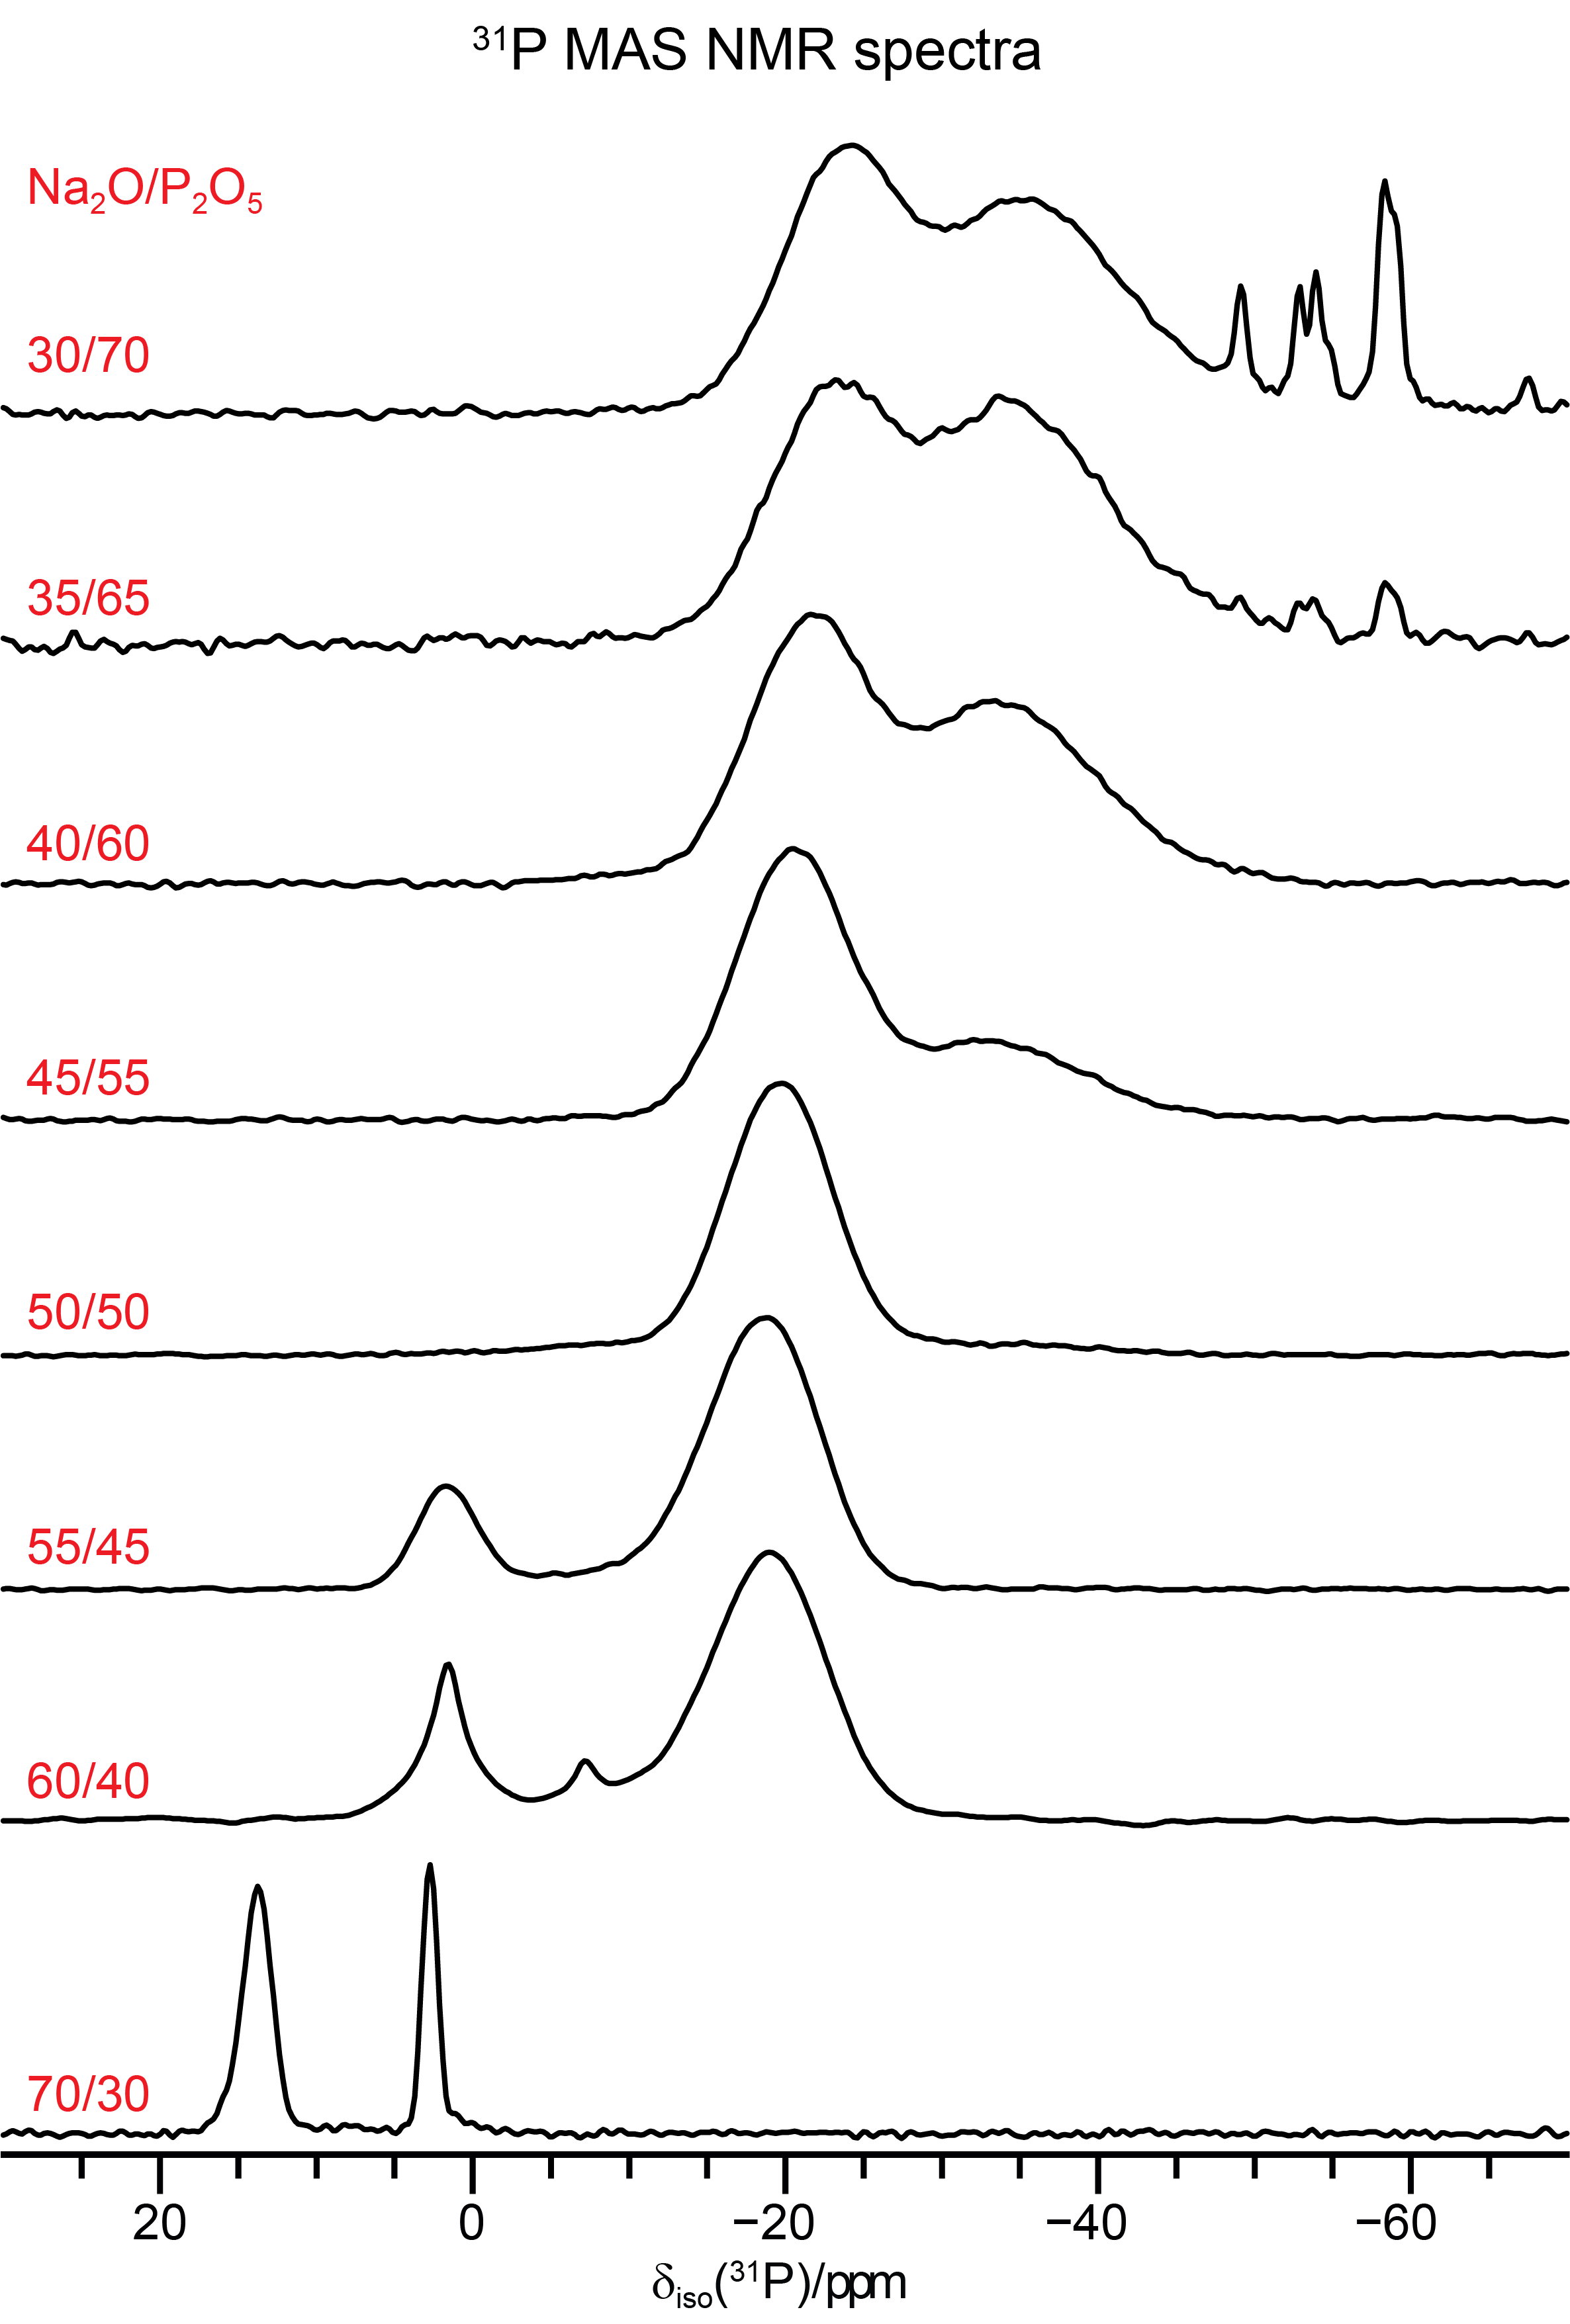
\includegraphics[scale=0.3]{NMR-spectra-2024-g1.png}
  \caption{Zeigt die NMR-Spektren der Verschieden Gläser}
  \label{nmrspektrums}
\end{figure}

\noindent
Die Integrale und Peak-Positionen sind in Tabelle \ref{peaks} zusammengefasst.
\newpage

\begin{table}
  \caption{Darstellung der unterschiedlichen Zusammensetzungen der Gläser in Kombination mit den jeweiligen \ce{^{31}P}-NMR-Peaks und den entsprechenden Integralen.}
  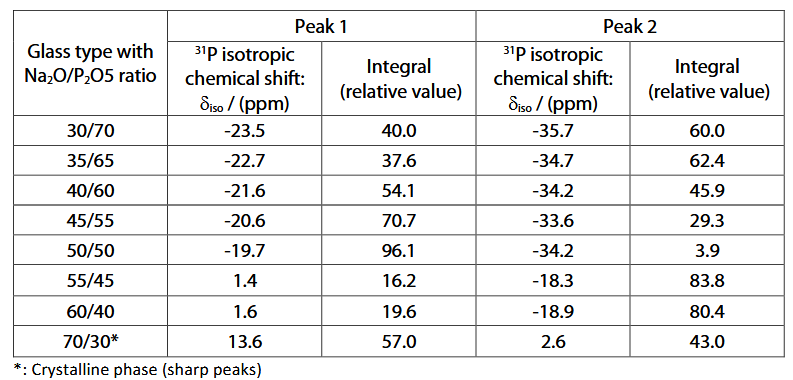
\includegraphics[width=\linewidth]{nmrpeaks.png}
  \label{peaks}

\end{table}
\noindent
Die in Tabelle \ref{peaks} aufgeführten Integrale dienen als Grundlage für die Berechnung der relativen Anteile der einzelnen Verknüpfungsgrade. Die Ergebnisse dieser Umrechnung sind in der 
Tabelle \ref{anteileee} zusammengefasst.

\begin{table}[!h]
  \caption{Zeigt den Anteil der Verknüpfungsgraden in Abhänigkeit der Zusammensetzung der Gläser.}
  \centering
  \begin{tabular}{|>{\centering\arraybackslash}p{4cm}|>{\centering\arraybackslash}p{2cm}|>{\centering\arraybackslash}p{2cm}|>{\centering\arraybackslash}p{2cm}|>{\centering\arraybackslash}p{2cm}|}
    \hline
    \rowcolor{lightgray}
    Zusammensetzung \ce{Na2O} / \ce{P2O5} [mol \%]&Anteil $Q^0$ [\%]&Anteil $Q^1$ [\%]&Anteil $Q^2$ [\%]&Anteil $Q^3$ [\%]\\
    \hline
    30 / 70&-&-&40&60\\
    \hline
    35 / 65&-&-&37.6&62.4\\
    \hline
    40 / 60&-&-&54.1&45.9\\
    \hline
    45 / 55&-&-&70.7&29.3\\
    \hline
    50 / 50&-&-&96.1&3.9\\
    \hline
    55 / 45&-&16.2&83.8&-\\
    \hline
    60 / 40&-&19.6&80.4&-\\
    \hline
    70 / 30&57.0&43.0&-&-\\
    \hline


  \end{tabular}
  \label{anteileee}
\end{table}

\noindent
Die Werte werden nun gegen den molaren Prozentanteil von \ce{Na2O} aufgetragen und mit den theoretischen Werten verglichen.
Dies wird in der Abbildung \ref{plot} dargestellt.
\newpage
\begin{figure}
  \centering
  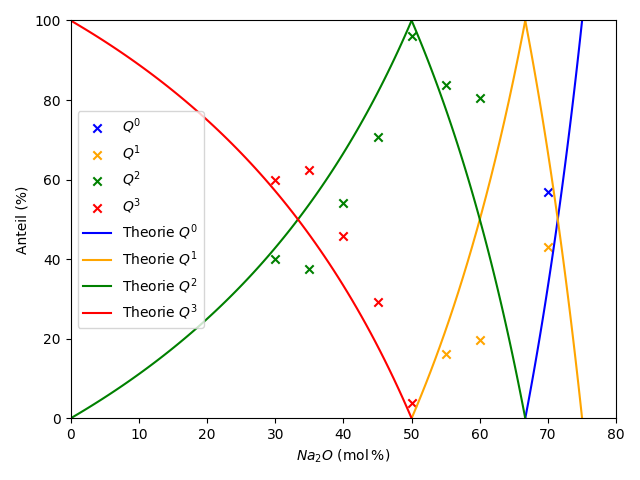
\includegraphics[scale=0.7]{plot.png}
  \caption{Dargestellt sind die Anteile des Verknüpfungsgrad Q in den hergestellten Gläsern im Vergleich zu den theoretischen Werten.\cite{Kirkpatrick.1995}}
  \label{plot}
\end{figure}

\noindent
Aus Abbildung \ref{plot} lässt sich ablesen, dass die Zusammensetzung der hergestellten Gläser im Wesentlichen den theoretischen Werten entspricht. Allerdings treten Abweichungen auf, die vermutlich auf Wägefehler zurückzuführen sind. Diese könnten die tatsächliche Zusammensetzung der Gläser beeinflusst haben, sodass der molare Prozentanteil von \ce{Na2O} nicht exakt dem in der Abbildung verwendeten Wert entspricht.
Zudem zeigt die Abbildung, dass der Anteil an $Q^3$-Einheiten mit abnehmender \ce{Na2O}-Konzentration zunimmt. Bei reinem \ce{P2O5} sind laut der theoretischen Kurve ausschließlich $Q^3$-Verknüpfungen zu erwarten, was mit der bekannten Struktur von \ce{P2O5} übereinstimmt.


\newpage
\section{Zusammenfassung}
Im Experiment wurden Gläsermit verschieden \ce{Na2O}-Anteilen zu \ce{P2O5} hergestellt. Diese wurden dann mit NMR- und XRD-Messungen untersucht.
Die XRD-Analyse zeigte für Gläser mit bis zu 60 mol \% \ce{Na2O} keine signifikanten Reflexe, was auf eine amorphe Struktur hinweist. Bei 70 mol \% \ce{Na2O} traten kristalline Reflexe auf, die der Phase \ce{Na3PO4} zugeordnet werden konnten.

\noindent
Zur genaueren strukturellen Charakterisierung wurde \ce{^{31}P}-NMR-Spektroskopie eingesetzt. Die daraus bestimmten chemischen Verschiebungen ermöglichten die Identifikation der verschiedenen Verknüpfungstypen ($Q^0$–$Q^3$) der \ce{PO4^{3-}}-Einheiten. Die relativen Integrale der Peaks wurden ausgewertet, um den Anteil jedes Q-Typs in Abhängigkeit vom \ce{Na2O}-Gehalt zu berechnen.

\noindent
Die experimentellen Ergebnisse zeigen insgesamt eine gute Übereinstimmung mit den theoretischen Erwartungen.\cite{Kirkpatrick.1995} Kleinere Abweichungen sind vermutlich auf Wägeungenauigkeiten zurückzuführen.



\newpage
\section{Literaturverzeichnis}
\printbibliography







\end{document}